\documentclass[a4paper, 12pt,twoside]{book}

% set the paper size and the margins
\usepackage[top = 2cm, bottom = 2cm, left = 2cm, right = 4cm ]{geometry}
\usepackage[showboxes]{textpos}
\setlength{\TPHorizModule}{10mm}
\setlength{\TPVertModule}{\TPHorizModule}
\TPMargin{2mm}
% set the header and the footnote
\usepackage{fancyhdr}
% Supress the hyphenation
\hyphenation{thatshouldnot} 
% for table and equations
\usepackage{tablefootnote}
\usepackage{amsmath,amsfonts,amsthm}
\usepackage{multirow}
\usepackage{hhline}
% make a wide hat for the least-squares regression line
 \usepackage{scalerel,stackengine}
\stackMath
\newcommand\reallywidehat[1]{%
\savestack{\tmpbox}{\stretchto{%
  \scaleto{%
    \scalerel*[\widthof{\ensuremath{#1}}]{\kern-.6pt\bigwedge\kern-.6pt}%
    {\rule[-\textheight/2]{1ex}{\textheight}}%WIDTH-LIMITED BIG WEDGE
  }{\textheight}% 
}{0.5ex}}%
\stackon[1pt]{#1}{\tmpbox}%
}
\usepackage[shortlabels]{enumitem}

% knitr packages
\usepackage[]{graphicx}
\usepackage[]{color}
%% maxwidth is the original width if it is less than linewidth
%% otherwise use linewidth (to make sure the graphics do not exceed the margin)
\makeatletter
\def\maxwidth{ %
  \ifdim\Gin@nat@width>\linewidth
    \linewidth
  \else
    \Gin@nat@width
  \fi
}
\makeatother

\definecolor{fgcolor}{rgb}{0.345, 0.345, 0.345}
\newcommand{\hlnum}[1]{\textcolor[rgb]{0.686,0.059,0.569}{#1}}%
\newcommand{\hlstr}[1]{\textcolor[rgb]{0.192,0.494,0.8}{#1}}%
\newcommand{\hlcom}[1]{\textcolor[rgb]{0.678,0.584,0.686}{\textit{#1}}}%
\newcommand{\hlopt}[1]{\textcolor[rgb]{0,0,0}{#1}}%
\newcommand{\hlstd}[1]{\textcolor[rgb]{0.345,0.345,0.345}{#1}}%
\newcommand{\hlkwa}[1]{\textcolor[rgb]{0.161,0.373,0.58}{\textbf{#1}}}%
\newcommand{\hlkwb}[1]{\textcolor[rgb]{0.69,0.353,0.396}{#1}}%
\newcommand{\hlkwc}[1]{\textcolor[rgb]{0.333,0.667,0.333}{#1}}%
\newcommand{\hlkwd}[1]{\textcolor[rgb]{0.737,0.353,0.396}{\textbf{#1}}}%
\let\hlipl\hlkwb
\usepackage{framed}
\makeatletter
\newenvironment{kframe}{%
 \def\at@end@of@kframe{}%
 \ifinner\ifhmode%
  \def\at@end@of@kframe{\end{minipage}}%
  \begin{minipage}{\columnwidth}%
 \fi\fi%
 \def\FrameCommand##1{\hskip\@totalleftmargin \hskip-\fboxsep
 \colorbox{shadecolor}{##1}\hskip-\fboxsep
     % There is no \\@totalrightmargin, so:
     \hskip-\linewidth \hskip-\@totalleftmargin \hskip\columnwidth}%
 \MakeFramed {\advance\hsize-\width
   \@totalleftmargin\z@ \linewidth\hsize
   \@setminipage}}%
 {\par\unskip\endMakeFramed%
 \at@end@of@kframe}
\makeatother


\definecolor{shadecolor}{rgb}{.97, .97, .97}
\definecolor{messagecolor}{rgb}{0, 0, 0}
\definecolor{warningcolor}{rgb}{1, 0, 1}
\definecolor{errorcolor}{rgb}{1, 0, 0}
\newenvironment{knitrout}{}{} % an empty environment to be redefined in TeX

\usepackage{alltt}


% packages will be used by the 'kable' package
\usepackage{booktabs}
\usepackage{longtable}
\usepackage{array}
\usepackage{multirow}
\usepackage[table]{xcolor}
\usepackage{wrapfig}
\usepackage{float}
\usepackage{colortbl} 
\usepackage{pdflscape}
\usepackage{tabu}
\usepackage{threeparttable}
\usepackage{threeparttablex}
\usepackage[normalem]{ulem}
\usepackage{makecell}
\usepackage{xcolor}
\IfFileExists{upquote.sty}{\usepackage{upquote}}{}

% define a color for highlight
\definecolor{asparagus}{rgb}{0.53, 0.66, 0.42}
\definecolor{babypink}{rgb}{0.96, 0.76, 0.76}
\definecolor{champagne}{rgb}{0.97, 0.91, 0.81}
\definecolor{forestgreen}{rgb}{0.13, 0.55, 0.13}
\definecolor{dollarbill}{rgb}{0.52, 0.73, 0.4}

\usepackage{tcolorbox}

\tcbset{width=0.9\textwidth,boxrule=0pt,colback=champagne,arc=0pt,
auto outer arc,left=0pt,right=0p}

\usepackage{hhline}

\usepackage{amsmath}

\setlength{\parindent}{0.5cm} 

\usepackage{siunitx}

%Chinese yen
\usepackage{stackengine}
\newcommand{\textyen}{\stackengine{-6pt}{=}{\large{\text{Y}}}{O}{c}{F}{T}{S}}

\setlength{\parindent}{0cm}

\begin{document}

%Deal with the headers of each chapter
\pagestyle{fancy}
\fancyhf{}
\renewcommand{\chaptermark}[1]{ \markboth{#1}{} }
\fancyhead[CE,CO]{\leftmark}
\fancyfoot[LE,RO]{\thepage}

\chapter{Hypothesis Test}
A report says the average yearly income of Chinese people is 74,318\textyen, but you suspect the average income is less than reported. Is your suspicion correct? In this chapter, we will learn how to solve this problem through \textbf{hypothesis test}.
\newpage

\section{Basics of Hypothesis Test}

  In order to test whether a given coin is fair or not, it is tossed 100 times, and resulted in 45 heads. Does this provides convincing evidence that this coin is not fair?\vspace{0.3cm}

\begin{itemize}
\item \textbf{Hypotheses}\vspace{0.3cm}

In the above setting, we have two contending \textbf{hypotheses} about the parameter $p$ , where $p$ is the probability of getting a head when this coin is tossed. One hypothesis is $\displaystyle{p=\frac{1}{2}}$, which means the coin is fair. The other one is $\displaystyle{p \ne \frac{1}{2}}$, which means the coin is not fair. The firs hypothesis is called \textbf{null hypothesis}, denoted as $\textbf{H}_0$, and the second one is called \textbf{alternative hypothesis}, denoted as $\textbf{H}_a$. They are written as 
$$\textbf{H}_0:\quad p=\frac{1}{2}$$
$$\textbf{H}_a:\quad p\ne\frac{1}{2}$$
\colorbox{babypink}{\parbox{0.9\textwidth}{
\textbf{Remark:}
\begin{itemize}
\item Usually, the $\textbf{H}_a$ is the hypothesis we want to seek evidence for.
 \item The hypotheses are about parameters. 
You can not set statements like $\reallywidehat{p} = \frac{1}{2}$, $\bar{x} = 0.6$ as hypotheses.
 \end{itemize}
}}
\vspace{0.3cm}

 The \textbf{hypothesis test} is the procedure to make decisions between the two hypotheses.\vspace{0.3cm}

In the above case, if $\textbf{H}_a$ is true, it can either be $p < \frac{1}{2}$ or $p > \frac{1}{2}$. This type of \textit{hypotheses test} is called \textbf{two-sided hypotheses test}.\vspace{0.3cm}

If the hypotheses are set as either of the following

$$\textbf{H}_0:\quad p=\frac{1}{2}, \qquad \textbf{H}_a:\quad p >\frac{1}{2}$$

$$\textbf{H}_0:\quad p=\frac{1}{2}, \qquad \textbf{H}_a:\quad p <\frac{1}{2}$$

the \textit{hypotheses test} is called \textbf{one-sided hypotheses test}.\vspace{0.6cm}

\colorbox{champagne}{\parbox{0.9\textwidth}{
\textbf{Juicy Pineapples}\vspace{0.3cm}

At the Hawaii Pineapple Company, managers are interested in the size of the pineapples grown in the company’s fields. Last year, the mean weight of the pineapples harvested from one large field was 31 ounces. A  different irrigation system was installed in this field after the growing season.  Managers wonder how this change will affect the mean weight of  pineapples grown in the field this year.\vspace{0.3cm}
\begin{enumerate}[(a)]
    \item State appropriate hypotheses for performing a significance test. Be sure to define the parameter of interest.
    \item Is this a \textbf{one-sided} or \textbf{two-sided} hypotheses test?
\end{enumerate}
}}
\newpage





\item \textbf{The reasoning of hypotheses test}\vspace{0.3cm}

Let's use the ``fair coin'' setting and the hypotheses are
$$\textbf{H}_0:\quad p=\frac{1}{2}$$
$$\textbf{H}_a:\quad p\ne\frac{1}{2}$$ 
Among the 100 tosses, 45 are head.\vspace{0.3cm}

How to choose between those two hypotheses? The reasoning is like:   if we assume the \textit{null hypotheses} is true, and we get a sample with the sample proportion $\hat{p}$ far away from $\displaystyle p= \frac{1}{2}$, then we have convincing evidence for $H_a$ and reject $H_0$. \vspace{0.3cm}

\textbf{In the following, $H_0$ is assumed to be true, with $p = 1/2$!!!}\vspace{0.3cm}


How to tell whether $\reallywidehat{p}$ is far away from $p$ or not? We have to resort to the sampling distribution of $\reallywidehat{p}$ when assuming $H_0$ is true. According to what we learned before, if certain conditions are met, $\reallywidehat{p}$ is approximately normally distributed. 
$$\reallywidehat{p} \sim N(\mu_{\reallywidehat{p}}, \sigma_{\reallywidehat{p}}), \qquad \mu_{\reallywidehat{p}} = p, \quad \sigma_{\reallywidehat{p}} = \sqrt{\frac{p(1-p)}{n}}$$     
    \begin{figure}[H]
    \centering
    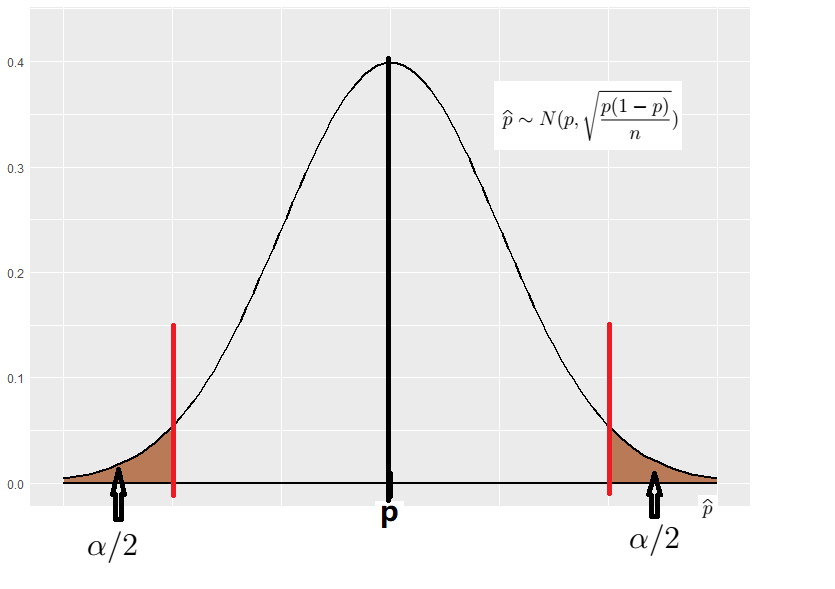
\includegraphics[scale=0.6]{HypothesisTestSamplingDistribution}
    \caption{$\hat{p}$ that is far away from $p$}
    \label{HypothesisTestSamplingDistribution}
    \end{figure}
    


In figure\ref{HypothesisTestSamplingDistribution}, we draw two lines away from $p$. If a $\reallywidehat{p}$ falls to the outside of those two lines, indicated by the shaded areas, we say this $\reallywidehat{p}$ is far away from $p$.\vspace{0.3cm}

However, where to draw those two lines? Referring to figure\ref{HypothesisTestSamplingDistribution}, if the total area of the ``shaded areas'' are given, then the position of the two lines are decided. We call this given total area \textbf{significance level $\mathbf{\alpha}$}. The most frequently used \textit{significance level} is $\mathbf{\alpha} = 0.05$.

\begin{textblock}{3}(15.5, -4)
\textblockcolor{dollarbill}
Set significance level $\mathbf{\alpha} = 0.05$. Is the $\reallywidehat{p}$ far away from $p$ in the case of ``fair coin'' with $$H_0 = 1/2$$ $$H_1 \ne 1/2$$
\end{textblock}
\vspace{0.3cm}

In the above \textit{two-sided hypotheses}, when $\reallywidehat{p}$ is either way larger or way smaller than $p$, we say $\reallywidehat{p}$ is far away from $p$ in the direction of $H_a$. Because, either ``way larger'' or ``way smaller'' is in favour of $H_a$.\vspace{0.3cm}

How to define ``far away'' in the case of \textit{one-sided hypotheses test}? Use the ``fair coin'' example, and change the hypotheses into 
    $$\textbf{H}_0:\quad p=\frac{1}{2}$$
$$\textbf{H}_a:\quad p\leq \frac{1}{2}$$ 

Since we have to decide whether  $\reallywidehat{p}$ is far away from $p$ in the direction of $H_a$, we have to draw a borderline to the left side of $p$, as shown in figure\ref{OneSidedHT}.    
     \begin{figure}[H]
     \centering
     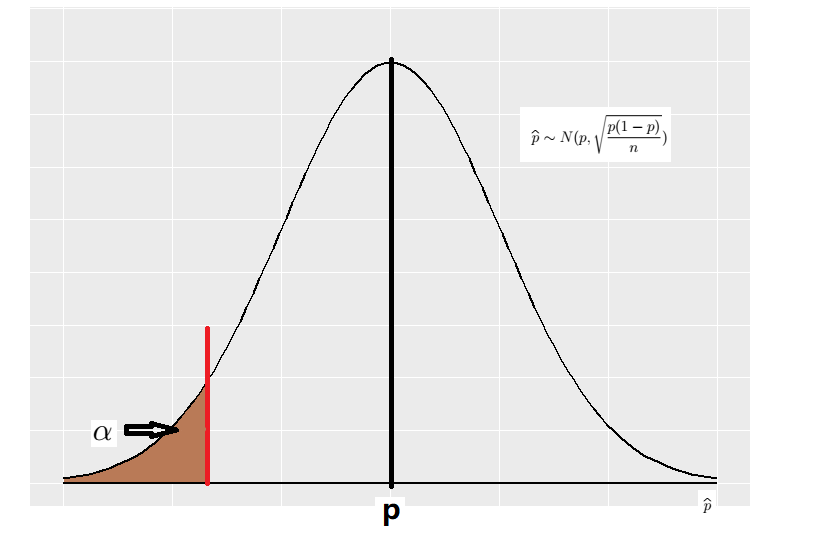
\includegraphics[scale=0.6]{OneSidedHT}
     \caption{One-sided hypotheses test}
     \label{OneSidedHT}
     \end{figure}
Here, the \textit{significance level} $\mathbf{\alpha}$ is the area to the left side of the borderline demarcating whether $\reallywidehat{p}$ is far away from $p$ or not.

\begin{textblock}{3.6}(-3, -4)
\textblockcolor{dollarbill}
Set significance level $\mathbf{\alpha} = 0.05$. Is the $\reallywidehat{p}$ far away from $p$ in the case of ``fair coin'' with $$H_0 = 1/2$$ $$H_1 \leq 1/2$$
\end{textblock}
\vspace{0.6cm}

In the case of \textit{one-sided hypotheses test} as
    $$\textbf{H}_0:\quad p=\frac{1}{2}$$
$$\textbf{H}_a:\quad p\leq \frac{1}{2}$$ 
everything is argued similarly.\vspace{0.6cm}

\colorbox{babypink}{\parbox{0.9\textwidth}{
\textbf{Remark:}\vspace{0.3cm}

 \begin{itemize}
     \item \textbf{Significance level $\alpha$ is set before the sample is drawn.} 
     \item \textbf{The hypotheses is set before the sample is drawn.}
     \item \textbf{All the above are based on the assumption that $H_0$ is true.}
 \end{itemize}

}}

\newpage

\item \textbf{The p-value}\vspace{0.3cm}

Still use the ``fair coin'' example, and the hypotheses are
$$\textbf{H}_0:\quad p=0.5$$
$$\textbf{H}_a:\quad p\ne0.5$$ 
The sample proportion $\reallywidehat{p} = 45/100 = 0.45$.\vspace{0.3cm}

Assume $H_0$ is correct. The probability 
$\textbf{P}(|\reallywidehat{p}-0.5| > |0.45-0.5|)$ are shown in figure



\end{itemize}






\newpage


 \colorbox{champagne}{\parbox{\textwidth}{
 \textbf{Calcium and Blood Pressure}\vspace{0.3cm}
 
 Does increasing the amount of calcium in our diet reduce blood pressure? Examination of a large sample of people revealed a relationship between calcium intake and blood pressure. The relationship was strongest for black men. Such observational studies do not establish causation. Researchers therefore designed a randomized comparative experiment.\vspace{0.3cm}
 
 The subjects were 21 healthy black men who volunteered to take part in the experiment. They were randomly assigned to two groups: 10 of the men received a calcium supplement for 12 weeks, while the control group of 11 men received a placebo pill that looked identical. The experiment was doubleblind. The response variable is the decrease in systolic (top number) blood pressure for a subject after 12 weeks, in millimeters of mercury. An increase appears as a negative number. Here are the data:
 \begin{table}[H]
 \centering
 \begin{tabular}{lcccc ccccc cc}
 \hline
 \textbf{Group 1 (calcium):}&7 &−4 &18 &17 &−3& −5 &1 &10 & 11& −2&\\
 \textbf{Group 2 (placebo):}&−1 &12 &−1 &−3 & 3 &−5& 5  &2& −11& −1 &−3\\
 \hline
 \end{tabular}
 \end{table}
 
 }}




\end{document}